\documentclass{beamer}

\usepackage[utf8]{inputenc}
\usepackage{graphicx} % Paquete para agregar graficos
\usepackage{multicol} % Paquete para agregar varias columnas
\usepackage{listings} % Paquete para agregar código
\usepackage{hyperref} % Paquete para agregar hiperlinks (NAVEGACIÓN A TRAVÉS DEL DOCUMENTO), como la imagen.
\usepackage{enumerate} % enumerados
\usepackage{verbatim} % comentarios
\usepackage{amsmath}
\usepackage[spanish]{babel}

\usetheme{Warsaw} % Tema de la presentación
\usecolortheme{seahorse}  % Colores de la presentación
\useoutertheme{shadow} % Aspecto de cabezal y pie de página
\usefonttheme{serif} % Estilo de la letra
\useinnertheme{rectangles} % Aspecto de listas y bloques

\graphicspath{ {Image/} }  %%  le indica a LaTeX que las imágenes están guardadas en una carpeta llamada Image bajo el directorio actual. 

% \ttfamily Mecanografia        \rmfamily   % Tipos de letra

\hypersetup{pdftitle= LaTeX, 
            pdfauthor=LeidyAldana,
            colorlinks=false,
            urlcolor=blue,
            pdfstartview=FitH,
            pdfpagemode=UseOutlines,
            pdfnewwindow,
            breaklinks
          }

\begin{document}

    % "Estoy convencido de que lo único que nos permite contemplar el mundo en que vivimos sin sentir repugnancia es la belleza que de vez en cuando el hombre crea a partir del caos. Los cuadros que pinta, la música que compone, la vida que lleva. De todas estas cosas, la más hermosa es una vida hermosa. Ésa es la obra de arte más perfecta."  W. Somerset Maugham, El velo pintado página 223


\begin{frame}
   
    \begin{center}
    
        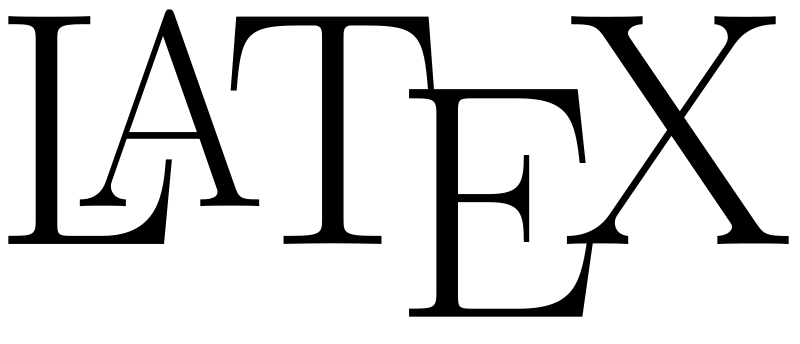
\includegraphics[width=6cm]{latex_logo.png}
           
         \vspace{0.4cm}
        %{ \ttfamily  \'Enfasis en redacción de \\artículos científicos y documentos. }
        Nivel básico en redacción de \\artículos científicos y documentos.\\
       \vspace{0.3cm}
        
        
\includegraphics[width=3.0cm]{GLUD.png}
        
\includegraphics[width=1.5cm]{escudo_ud_blanco_y_negro}
        
\includegraphics[width=2.5cm]{IISE.png}
    
    \end{center}

\end{frame}

    % ¿Qué es LaTeX? y su historia
    
\begin{frame}
   TeX, programa de composición tipográfica \\(1997, Donald Knuth)
   \begin{itemize}
        \item LaTeX, Software Libre \\Sistema de preparaci\'on de documentos derivado de TeX
        \item Creado en 1985 por Leslie Lamport\footnote{1941, Científico Informático Estadounidense}
        \vspace{1.5cm}
        \begin{enumerate}
            \item Compilado, hace uso de etiquetas
            \item Documento en lugar del diseño.
            \item Información cabecera $\rightarrow$ maqueta el texto.
            \item Genera un pdf con calidad profesional.
        \end{enumerate}
    \end{itemize}    
\end{frame}

    
    % ¿Qué se necesita para elaborar algo en LaTeX?
    \begin{frame}
    \textbf{Componentes}
        \begin{itemize}
            \item Editor de Texto
            \item Distribuci\'on \TeX{}
            \item Visor de Documentos
        \end{itemize}
        \vspace{2.0cm}
        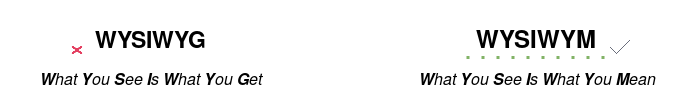
\includegraphics[width=\textwidth]{WYSWY}
\end{frame}

    
    % Proceso de compilación
    \begin{frame}
    \frametitle{Compilando \LaTeX{}}
    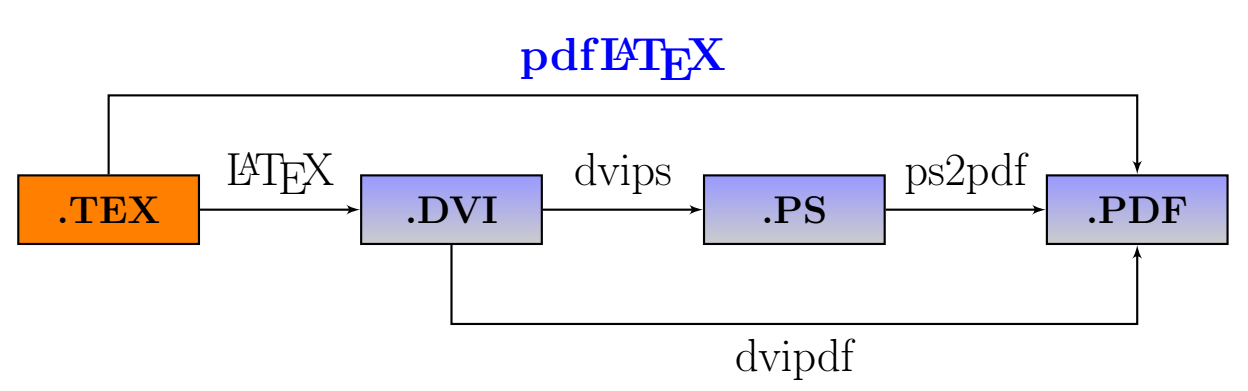
\includegraphics[width=\textwidth]{compilado.png}  
\end{frame}


    \begin{frame}
   \frametitle{Compilando \LaTeX{}}
   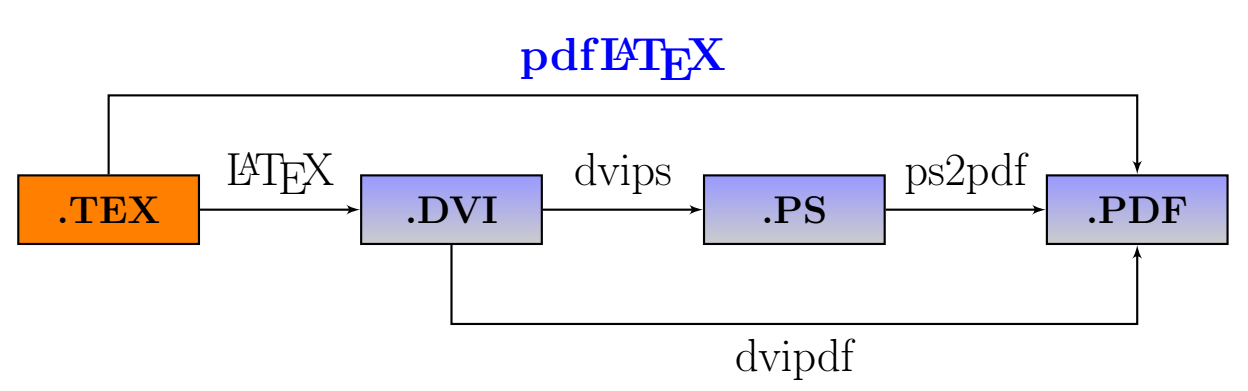
\includegraphics[width=\textwidth]{compilado.png}
   \vspace{0.9cm}\\
    \centering
    \begin{exampleblock}{Primera opci\'on en el proceso de compilaci\'on} % MARCO width=8cm, height=3cm
        {\ttfamily \$ latex informe.tex\\ 
                          \$ dvips informe.dvi -o informe.ps \\
                          \$ ps2pdf informe.ps  }                               
    \end{exampleblock}                                  
\end{frame}


    \begin{frame}
   \frametitle{Compilando \LaTeX{}}
   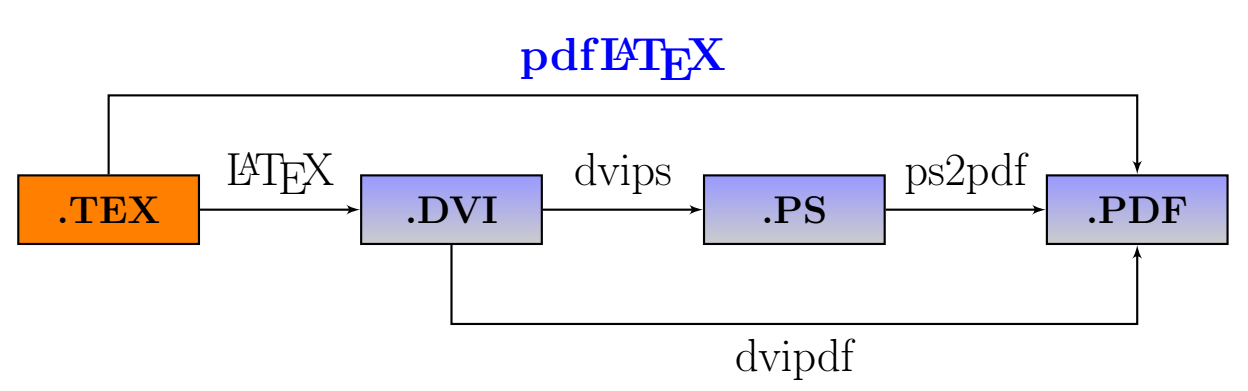
\includegraphics[width=\textwidth]{compilado.png}
   \vspace{0.9cm}\\
    
            \centering
            \begin{exampleblock}{Segunda opci\'on en el proceso de compilaci\'on} % MARCO width=8cm, height=3cm
                {\ttfamily \$ pdflatex informe.tex }                                       
            \end{exampleblock}            
            %\rule{100pt}{150pt}% Place your graphic here
       
        
       
\end{frame}


    \begin{frame}
   \frametitle{Compilando \LaTeX{}}
   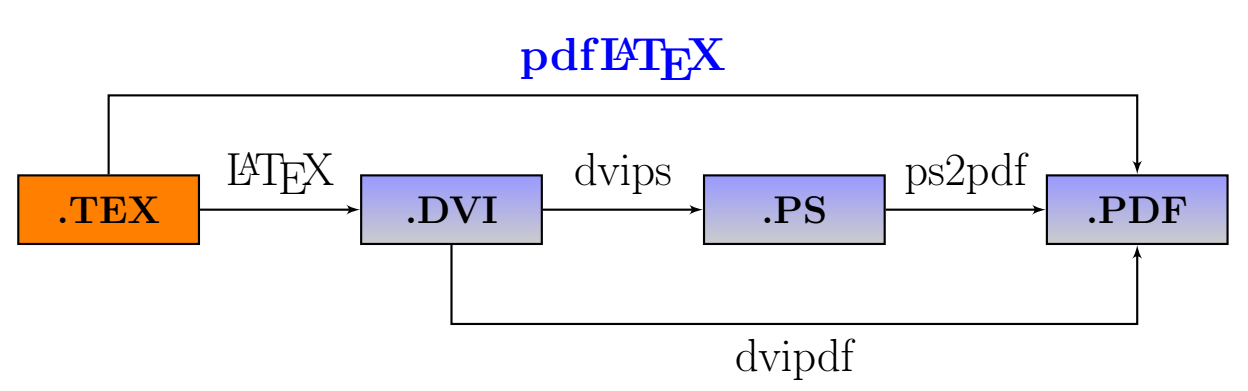
\includegraphics[width=\textwidth]{compilado.png}
   \vspace{0.9cm}\\
    
            \centering
            \begin{exampleblock}{Tercera opci\'on en el proceso de compilaci\'on} % MARCO width=8cm, height=3cm
                {\ttfamily \$ latex informe.tex\\ 
                           \$ dvipdf informe.dvi   }                       
                
            \end{exampleblock}            
            %\rule{100pt}{150pt}% Place your graphic here
\end{frame}


    
    % Ingreso a un entorno de desarrollo virtual
    %\begin{frame}
 
%   
\includegraphics[width=6.0cm]{MakeDocument}
   
%\end{frame}


\begin{frame}
   \frametitle{Creando un documento...}
   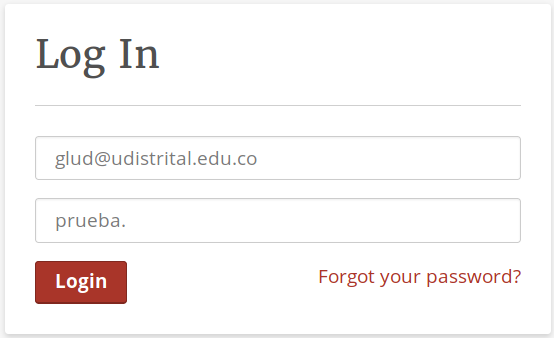
\includegraphics[width=\textwidth]{login}\footnote{\url{https://www.sharelatex.com/login}}
   
\end{frame}


    %- convertir un documento sencillito de word a LaTeX,
% estructurarlo como artículo, o como libro
% ecuaciones $$, cartas y presentaciones en LaTeX, así como a incorporar fuentes, colores, y gráficos.

\begin{frame}{}
     \begin{columns}[onlytextwidth]
        \begin{column}{0.48\textwidth}            
            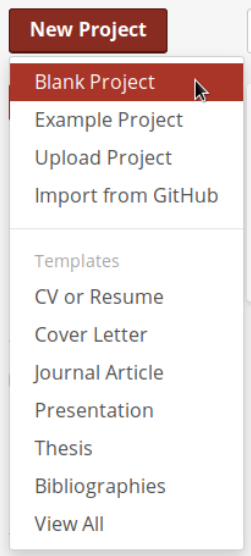
\includegraphics[width=4.0cm]{sh1}          
        \end{column}        
        \begin{column}{0.48\textwidth}            
            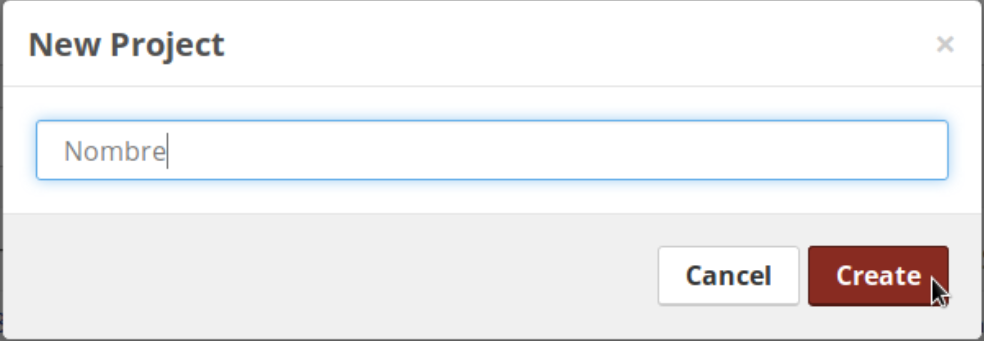
\includegraphics[width=6.0cm]{New}
        \end{column}
\end{columns} 
    
    
    
    


\end{frame}

    % Inicio del documento (tipoDocumento, tipos, ManejoDeAlgunasCosas)
    \begin{frame}
    
    \textbackslash documentstyle[12pt]\{article\};
         
    
\includegraphics[width=\textwidth]{type}\\   
    % matriz para elegir el formato y combinación de colores https://www.hartwork.org/beamer-theme-matrix/
   
    \begin{itemize}    
        \item Etiquetas con inicio y fin.
        \item Secciones, subsecciones y enumeración.
        \item Tabla de contenidos        
    \end{itemize}
    
        Secciones sin enumerar en la tabla de contenidos!
    
\end{frame}


    % Caracteres especiales, 
    \begin{frame}
    ¡Colocar \textit{backslash} para caracteres especiales! \\
    \# , \$ , \% , \& , \_ , \{ , \} , \^  , ~ \textbackslash \\
    % Espacio vertical  
    %\vspace{2.0cm}
    \begin{flushright}
        \href{https://www.ctan.org/lion/}{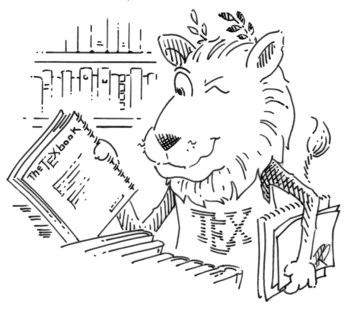
\includegraphics[width=3.0cm]{lion}} 
    \end{flushright}
    \textbackslash textbf\{\} : coloca el texto en negrilla : Ctrl+b \\
    \textbackslash textit\{\} : coloca el texto en cursiva : Ctrl+i \\
    \textbackslash footnote\{\} : pie de página
    
    
   
\end{frame}
    
    \begin{frame}{}
    \begin{itemize}
        \item \textbackslash usepackage\{ graphicx\}, cargar paquetes que añaden nuevas funcionalidades a LaTeX\footnote{\url{http://metodos.fam.cie.uva.es/~latex/curso-2015/apuntes3.pdf}
        \item Referencias, tablas, figuras
        \item Expresiones Matemáticas
        \item $\sqrt[4]{5}$
        \item Bibliografías e índices
        \item Columnas e Imágenes, \textit{eps png jpg}
    \end{itemize}
    
\end{frame}
    \begin{frame}
    \frametitle{Listas en \LaTeX{}}

    \begin{columns}[onlytextwidth]
        \begin{column}{0.48\textwidth}
            \centering
            \begin{exampleblock}{Con un guión definido} % MARCO width=8cm, height=3cm
                \begin{itemize}
                    \item[$*$] Madrid.
                    \item Castilla la Mancha.
                    \item Castilla y León.
                    \begin{itemize}
                        \item Segovia.
                        \item Ávila.
                    \end{itemize}
                \end{itemize}
            \end{exampleblock}
        \begin{exampleblock}{Con un guión definido} % MARCO width=8cm, height=3cm    
            \begin{enumerate}[1.]
                \item Manzanas.
                \item Plátanos.
                \item Pescado fresco.
                \begin{enumerate}[a)]
                    \item Emperador.
                    \item Gallo.
                \end{enumerate}
            \end{enumerate}
        \end{exampleblock}      
            %\rule{100pt}{150pt}% Place your graphic here
        \end{column}
        
        \begin{column}{0.46\textwidth}
            \begin{exampleblock}{} %marco tipo block
                \begin{description}
                    \item[Australia:] Canguro.
                    \item[EEUU:] Águila calva.
                    \item[España:] Toro.
                    \item[México:] Águila real.
                \end{description}
            \end{exampleblock}
        \end{column}
    \end{columns} 
\end{frame}


% \usepackage{hyperref}
%   para colocar hipervinculos
%\href{url}{http://www.texample.net/tikz/resources/}

%   Above = antedicho, encima, arriba, encima de


\begin{comment}
%-------------- ENUMERACION

\begin{itemize}
    \item[$*$] Madrid.
    \item Castilla la Mancha.
    \item Castilla y León.
    \begin{itemize}
        \item Segovia.
        \item Ávila.
    \end{itemize}
\end{itemize}
___________________________________

\begin{enumerate}[1.]
    \item Manzanas.
    \item Plátanos.
    \item Pescado fresco.
    \begin{enumerate}[a)]
        \item Emperador.
        \item Gallo.
    \end{enumerate}
\end{enumerate}

__________________________________-

\begin{description}
    \item[Australia:] Canguro.
    \item[EEUU:] Águila calva.
    \item[España:] Toro.
    \item[México:] Águila real.
\end{description}

\end{comment}




%  \includegraphics[width=\textwidth]{ //NOMBRE DE LA IMAGEN }   == linea para añadir imagenes gracias a la librería.

% "  " \par aplica Sangría

%  \textcolor{red}{Hola} == coloca el texto en color.


% "En el mundo del código abierto, la vergüenza es uno de los principales factores de motivación hacia el aumento de la calidad de su código!)" 
% página 34, Software libre para una sociedad libre

    
    %\begin{frame}
    \frametitle{Compilando \LaTeX{}}

    \begin{columns}[onlytextwidth]
        \begin{column}{0.48\textwidth}
            \centering
            \begin{exampleblock}{Editable} % MARCO width=8cm, height=3cm
                \begin{center}
                    \begin{enumerate}                        
                        \item { \ttfamily \$ latex informe.tex}
                        \item { \ttfamily \$ pdflatex informe.tex}
                    \end{enumerate}                                     
                \end{center}
            \end{exampleblock}
            \begin{enumerate}
                \item { \ttfamily informe.aux  informe.dvi  informe.log}
                \item { \ttfamily  informe.aux  informe.log  informe.pdf}
            \end{enumerate}
            
            %\rule{100pt}{150pt}% Place your graphic here
        \end{column}
        
        \begin{column}{0.46\textwidth}
            \begin{exampleblock}{} %marco tipo block
                \begin{itemize}
\item  Relación de uso más indicada cuando es necesaria una asociación entre clases pero el \textit{principio de Liskov} no se cumple
\item  Herencia múltiple manual (composición de objetos). 
%\includegraphics[width=\textwidth]{Caja.png}
\item  Usado en Patrones de diseño como \textit{Strate, Strategy, Visitor}

\item %Caracterizado por la reutilización selectiva
Utilizando interface, la delegación puede hacerse de manera más flexible y fuertemente tipada
\end{itemize}

\end{exampleblock}
\end{column}
\end{columns} 
\end{frame}


    %

\begin{frame}
   \frametitle{\textbf{Compilando \LaTeX{} }}
 
\begin{columns}[onlytextwidth]
    \begin{column}{0.34\textwidth}
     \centering
     { \ttfamily informe.tex }  \\
     (Puede ser editado a través de cualquier editor de texto)
   \begin{exampleblock}{Definición} % MARCO width=8cm, height=3cm
    \begin{center}
        Patrón en el que una clase muestra un comportamiento pero delega la responsabilidad de implementar ese comportamiento a otra clase. 
   \end{center}
    \end{exampleblock}
   
      %\rule{100pt}{150pt}% Place your graphic here
      
    \end{column}
    \begin{column}{0.56\textwidth}
    \begin{exampleblock}{} %marco tipo block

 \begin{itemize}
 \item  Relación de uso más indicada cuando es necesaria una asociación entre clases pero el \textit{principio de Liskov} no se cumple
        \item  Herencia múltiple manual (composición de objetos). 
        %\includegraphics[width=\textwidth]{Caja.png}
        \item  Usado en Patrones de diseño como \textit{Strate, Strategy, Visitor}
        
        \item %Caracterizado por la reutilización selectiva
        Utilizando interface, la delegación puede hacerse de manera más flexible y fuertemente tipada
    \end{itemize}

    \end{exampleblock}
    \end{column}
  \end{columns} 
\end{frame}




\end{document}



% 'porque usar latex?
%http://nokyotsu.com/latex/guia.html